\documentclass{article}

\usepackage{amsmath}
\usepackage[margin=0.1in]{geometry}
\usepackage{booktabs}
\usepackage{tipa}
\usepackage{amssymb}
\usepackage{tikz}
\usetikzlibrary{fit}
%\usepackage{color}
\usepackage[dvipsnames]{xcolor}
\usepackage{multirow}
\usepackage{hyperref}

 % For algorithms
\usepackage{algorithm}
\usepackage{algorithmic}

\title{Discovering the Rules of language using Bayesian Program Learning}
%\author{Kevin Ellis, Timothy O'Donnell}

\newcommand{\nextForm}[1]{\rotatebox[origin=c]{270}{$_{\curvearrowright}$}$_{#1}$}
\DeclareMathOperator*{\argmin}{arg\,min}

\begin{document}
\maketitle


%% How do linguists come up with phonological rules, how do kids learn
%% artificial grammars, and how does one acquire pig latin?  The
%% solutions to these problems share a common representation, which we
%% show can be modeled as a program, and the corresponding learning
%% problems modeled as program induction.  This framing lets us apply
%% ideas from Bayesian Program Learning to induce grammars, which
%% combines program synthesis techniques with a compression-based inductive
%% bias. This lets the models capture phonological phenomena like vowel
%% harmony or stress patterns and learn synthetic grammars used in prior
%% studies of artificial grammar learning.  Going beyond individual
%% grammar learning problems, we consider the problem of jointly
%% inferring many related rule systems. By solving many textbook
%% phonology problems, we can ask the model what kind of inductive bias
%% best explains the attested phenomena.


\begin{abstract}
    %% How do linguists come up with phonological rules? How do kids
    %% learn pig latin?  We develop computational models of these and
    %% other phenomena in language.  The unifying element of the models
    %% is to treat grammars as programs, which lets us apply ideas from
    %% the field of program synthesis to learn grammars. This lets the
    %% models capture phonological phenomena like vowel harmony or stress
    %% patterns and learn synthetic grammars used in prior studies of
    %% rule learning.  Going beyond individual grammar learning problems,
    %% we consider the problem of jointly inferring many related rule
    %% systems. By solving many textbook phonology problems, we can
    %% ask the model what kind of inductive bias best explains the
  %% attested phenomena.
Both children and linguists confront a similar problem of inference:
given utterances produced by speakers, together with aspects of the
meaning of those utterances, discover the grammatical principles that
relate form to meaning. We study this abstract computational
problem within the domain of morphophonology, contributing a computational model
that learns phenomena from many natural languages and generalizes in
humanlike ways from data used in behavioral studies of artificial grammar
learning.

Our work draws on two analogies. The \emph{child-as-linguist analogy}
holds that both children and linguists must solve the same abstract
inductive reasoning problem, even though the nature of the input data and underlying mental algorithms
are surely different in precise detail. Accordingly we isolate the
problem of learning morphophonological systems, and show that a single
solution to this problem can capture both linguistic analyses from
natural languages and infant rule learning of artificial languages.
We adopt the framework of ``Bayesian Program learning'' (BPL) -- in
which learning is formulated a synthesizing a program which compactly
describes the input data. This \emph{learning-as-programming analogy}
lets us exploit recent techniques from the field of program synthesis to
induce morphophonological rules from data.
While \emph{child-as-linguist} poses the
computational problem, \emph{learning-as-programming} offers a
solution.
  \end{abstract}

\section{Introduction}

Both children and linguists confront a similar problem of inference:
given utterances produced by speakers, together with aspects of the
meaning of those utterances, discover the grammatical principles that
relate form to meaning. Here, we study this abstract computational
problem within the domain of morphophonology, the part of language
that builds up words from simpler parts such as stems, prefixes, and
suffixes (morphology) and then specifies how the words are realized as
sound patterns (phonology).  Our contribution is a computational model
that learns phenomena from 26 natural languages and generalizes in
humanlike ways from data used in infant studies of artificial grammar
learning.

Our work draws on two analogies. The \emph{child-as-linguist analogy}
holds that both children and linguists must solve the same abstract
inductive reasoning problem, even though the nature of the input data,
the process of theory construction, and underlying mental algorithms
are surely different in precise detail. Accordingly we isolate the
problem of learning morphophonological systems, and show that a single
solution to this problem can capture both linguistic analyses from
natural languages and infant rule learning of artificial languages.

We adopt the framework of ``Bayesian Program learning'' (BPL) -- in
which learning is formulated a synthesizing a program which compactly
describes the input data. This \emph{learning-as-programming analogy}
explains the flexibility and richness of a grammar
as a consequence of 
While \emph{child-as-linguist} poses the
computational problem, \emph{learning-as-programming} offers a
solution.

We develop a programming language tailored to expressing
morphophonological generalizations.
For children this programming language is innate and is
commonly called ``Universal Grammar'' (UG). Linguists instead must
uncover this programming language by looking at many languages and
searching for commonalities. Learning what makes up UG unfolded over
evolutionary time for children and is ongoing within linguistics.  BPL
reinterprets the problem of discovering UG.  In BPL, UG is the
programming language combined with an inductive bias over programs.
Here we estimate this inductive bias empirically from naturally
occurring morphophonological systems as a way of learning to learn
grammars.

\section{Morphophonological phenomena}

What is phonology supposed to explain? Familiar phenomena from
English help motivate phonological grammars.  The plural of \emph{cat}
is pronounced \textipa{k\ae ts} (``cats''), while the plural of
\emph{dog} is pronounced \textipa{dagz} (``dogs''). A phonological
rule accounts for the alternation between \textipa{s} and \textipa{z}:
\textipa{z} becomes \textipa{s} at the end of words whenever the
preceding sound is unvoiced (does not involve vibrating the vocal
cords). This generalization holds throughout the entirety of English.
The count system of Tibetan presents another puzzle.
``1'' in Tibetan is pronounced
\textipa{\|x{j}ig}, ``10'' is \textipa{\|x{j}u},
yet ``11'' ($ = 10 + 1$) is \textipa{\|x{j}ug\|x{j}ig},
rather than \textipa{\|x{j}u\|x{j}ig}.
The explanation lies in Tibetan phonology,
which deletes word initial consonants followed by another consonant (Table~\ref{Tibetan}).
In this analysis of Tibetan,
``1'' has a latent ``underlying'' representation as \textipa{g\|x{j}ig}
but is pronounced as \textipa{\|x{j}ig}.

The aim of phonology is to explain pronunciations of words in terms of
latent underlying representations (eg, \textipa{g\|x{j}ig} for Tibetan
``1'') and the rules that give observed surface pronunciations from
underlying forms (eg, deleting word initial consonants).
Context-sensitive rewrite systems are a Turing complete representation
that also naturally express phonological
rules~\cite{chomsky1968sound}.  We use context-sensitive rewrites as a
representation for programs that implement a language's phonology.
For example, the rewrite in Table~\ref{Tibetan},
\verb|C|$\to\varnothing /$\verb|#_C|, deletes ($\to\varnothing $)
consonants (\verb|C|) at word boundaries (\verb|#|) when followed by
another consonant (\verb|C|).
Thus phonological rule learners, whether they be children, linguists, or machines, must solve a program induction problem.

\subsection{Inducing Programs}
We model the program learning problem as Bayesian inference, treating the pronunciations of words as observed data and the phonology as a latent variable whose values are programs. So the model's beliefs about possible programs are:
\begin{equation}
  P(\text{program}|\text{words})\propto P(\text{program}|\text{UG})\prod_{w\in\text{words}}\sum_{u\in\text{underlying forms}} P(u)P(w|u,\text{program})
  \end{equation}
Here, Universal Grammar (UG) is an inductive bias over programs. This inductive bias encodes knowledge of the program space (what rules are possible in human language and what rules are impossible), imparting a bias towards more naturally structured rules, like rules written in terms of syllables and consonants.

\subsection{The role and importance of universal grammar}
                We claim any plausible theory of linguistic rule learning needs a universal grammar. Studies of infant grammar learning suggests that babies come equipped with prior knowledge of what language should look like. This prior knowledge constrains the space of allowed generalizations, accounting for the astonishing pace at which children acquire language. This line of reasoning is a ``poverty-of-the-stimulus'' style argument: if children can induce so much grammar from such meager data, something else must bridge the gap. Because universal grammar also constrains the space of allowed grammars, we would expect that humans do not learn certain generalizations, even when the generalizations seem to hold in the data. Indeed this is the case: this ``surfeit-of-the-stimulus'' style argument  explains phenomena in natural languages (for example, statistical regularities that seem to hold in Turkish are not actually used by speakers) and in infant artificial language learning (for example, infants acquire certain phonological generalizations from just a few examples, while never acquiring other generalizations that are seemingly just a simple). While previous accounts of universal grammar were abstract, our model is concrete and computational. We define universal grammar as a probability mass function that puts zero mass on impossible or unattested generalizations, places more mass on programs licensing the generalizations that people learn quickly and naturally, and then smoothly falls off in probability mass as the programs become less natural.

\subsection{Learning natural language phonology}                
Our model learns a diverse set of phonological generalizations found in natural languages. We compiled a multilingual data set of words from standard linguistic textbooks. In these data sets, our model recovers allophonic relationships (e.g., l vs. r in Japanese) and systems that form different inflections of words (e.g., English verb inflections, or the Tibetan count system). Systems like these have received intense study within computational linguistics. But no prior model could explain the diversity of phonological phenomena found even in a textbook. To explain many diverse phenomena we need a rich, flexible representation -- programs -- coupled to a linguisticly informed inductive bias -- universal grammar. Our model learns simple generalizations like English verbal inflections, as well as phenomena like vowel harmony (in the language Kikuria, the word tiga becomes tegera in a different inflection, or ruga becomes rogera), or tonal rules in languages with tone (in the language Kerewe, different inflections cause tones to appear, disappear, or move to different parts of a word).

For these results, the learning-as-programming analogy does the work for us. BPL moves beyond the impoverished representations of prior learners (neural networks as in, or rigid classes of symbolic rules as in) instead represented generalizations as programs. We claim that programs are a sufficiently general representation to support the kinds of rules found in phonology.

                



\begin{table}\centering
\begin{tabular*}{10cm}{lcl}
  \toprule
  Example data&Phonology\\\midrule
\begin{tabular}{ll}
1&\textipa{\|x{j}ig}\\
4&\textipa{\|x{s}i}\\
5&\textipa{Na}\\
9&\textipa{gu}\\
10&\textipa{\|x{j}u}\\
11 ($= 10 + 1$) & \textipa{\|x{j}ug\|x{j}ig}\\
14 ($= 10 + 4$) & \textipa{\|x{j}ub\|x{s}i}\\
15 ($= 10 + 5$) & \textipa{\|x{j}uNa}\\
19 ($= 10 + 9$) & \textipa{\|x{j}urgu}\\
40 ($= 4 + 10$) & \textipa{\|x{s}ib\|x{j}u}\\
50 ($= 5 + 10$) & \textipa{Nab\|x{j}u}\\
90 ($= 9 + 10$) & \textipa{gub\|x{j}u}
\end{tabular}
&
\begin{tabular}{l}
  \emph{Consonant cluster reduction:}\\
  \verb|C|$\to\varnothing $ $/$ \verb|# _ C|\\
  \end{tabular}

  \\
  \bottomrule  \end{tabular*}
\caption{Tibetan count system.}
\label{Tibetan}
  \end{table}

\pagebreak


%% 2 insights: analogy between children and linguists. analogy between
%% grammars and programs.

%% The core problem we're pushing on is \textbf{structure learning in
%%   language}. It makes sense that you could learn parameters and
%% lexical items, but could you learn something with more the structure
%% of a grammar? Here we answer that question in the affirmative within a
%% restricted domain (phonology) on restricted problems (smaller data
%% sets and simpler sets of rules).

%% Why focus on some problems that feel more like computational linguistics and other problems that feel more like developmental psychology? Connection to child-as-linguist~\cite{chomsky1988current}, child-as-scientist, child-as-hacker\cite{Rule2015RepresentingAL}.

%% What is the connection between what children do and what linguists do? From the point of view of this research project,
%% the difference lies in the nature and role of universal grammar.
%% For a linguist, universal grammar is an unknown to be discovered.
%% When analyzing a new data set, a linguist might need to entertain a broader or more expressive universal grammar.
%% For the child, universal grammar is an innate part of our genetic endowment.



\section{The Model}

\begin{figure}[h!]\centering
  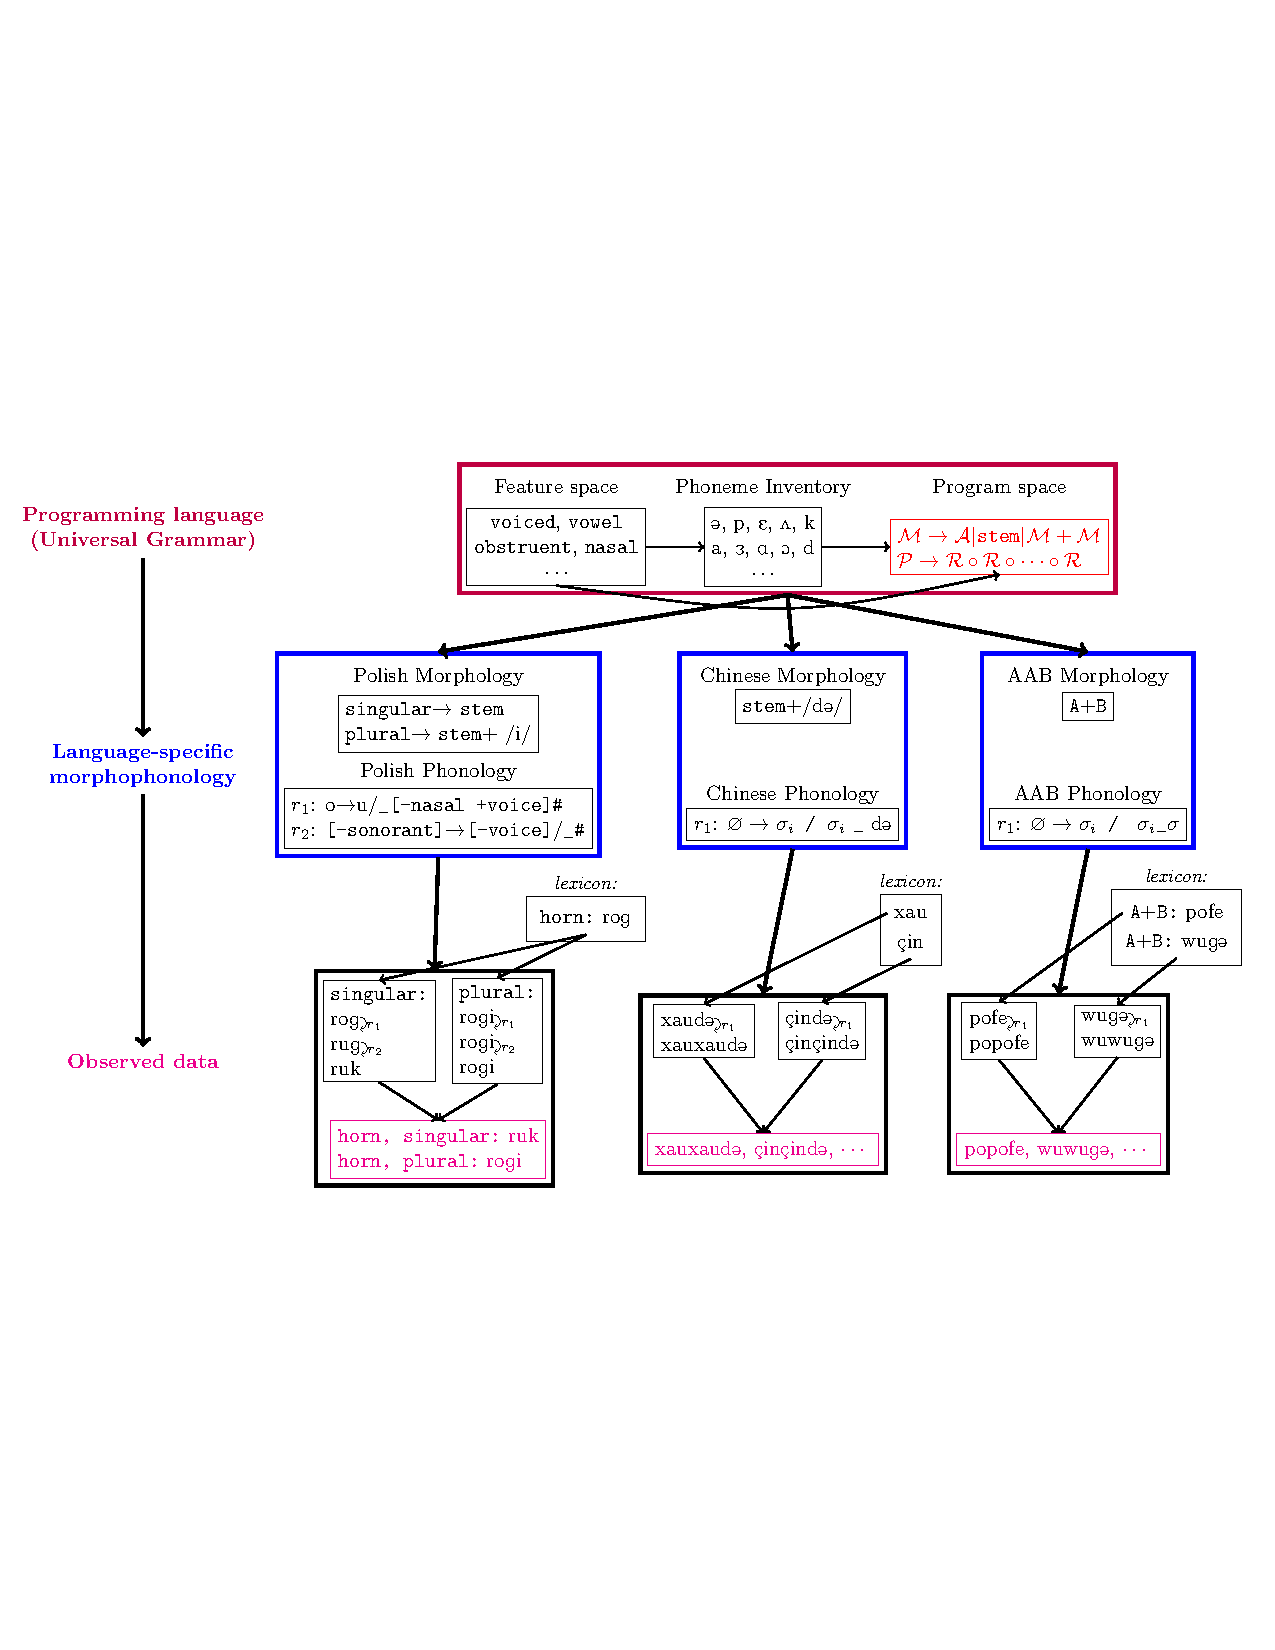
\includegraphics[width = 0.9\textwidth]{generativeModel.pdf}
  \caption{{\color{red}Red}: Both the morphology $\mathcal{M}$ and
    phonology $\mathcal{P}$ are programs either build through
    concatenation or function composition
    (Tables~\ref{morphologyGrammar} \&~\ref{phonologyGrammar}). These programs explain how words are built in both natural and artificial grammars ({\color{blue}blue}). Learners observe pronunciations of words ({\color{magenta}}) in order to recover these programs, but with the aid of a strong inductive bias (Universal Grammar, {\color{purple}purple})}.
  \label{beautiful}
\end{figure}

\section{Artificial Grammar Learning}

The fundamental hypothesis underlying AGL research is that
artificial grammar learning must engage some shared resource with first language acquisition --
and so we can gain insights into first language acquisition by
instead studying AGL in controlled experiments.

Our contribution to AGL research is the demonstration that
a single BPL model can explain (1) that infants quickly acquire
certain simple grammars very easily, and at the same time (2)
those same infants go on to learn
the very complicated grammar of their first language.
We collected grammars from AGL datasets~\cite{gerken2010infants,marcus1999rule,frank2011three}
and presented our BPL learner with data drawn from these grammars (Table~\ref{artificialGrammarTable}),
finding that our model recovers the generative processes that
 underlies these data sets.
\begin{table}[h!]
\centering\begin{tabular}{lcll}
  \toprule
  Grammar&Example input to learner&MAP grammar&Natural language analogues\\\midrule
  \begin{tabular}{l}
    ABA (same/different/same)\\
  Marcus et al. 1999.     
    \end{tabular}&
  \begin{tabular}{l}
    wofewo\\
    lovilo\\
    fimufi
  \end{tabular}&
  \begin{tabular}{l}
$\varnothing\to \sigma_i$\verb| / #_|$\sigma \sigma_i$
  \end{tabular}& Reduplication (eg, Tagalog)
  \\\midrule
  \begin{tabular}{l}
      ABB (different/same/same)\\
  Marcus et al. 1999. 
    \end{tabular}&
  \begin{tabular}{l}
        wofefe\\
    lovivi\\
    fimumu
  \end{tabular}&
  \begin{tabular}{l}
$\varnothing\to \sigma_i$\verb| / |$\sigma_i$\verb|_#|
  \end{tabular}&
  Reduplication (eg, Tagalog)\\\midrule
  \begin{tabular}{l}
      ABx (different/different/constant)
    \end{tabular}&
  \begin{tabular}{l}
        wofeka\\
    lovika\\
    fimuka
  \end{tabular}&
  \begin{tabular}{l}
stem$ + x$
  \end{tabular}&concatenative morphology
  \\\midrule
  \begin{tabular}{l}
    AAx (same/same/constant)\\Gerken 2006. %~\cite{gerken2010infants}
    \end{tabular}&
  \begin{tabular}{l}
        wowoka\\
    loloka\\
    fifika
  \end{tabular}&
  \begin{tabular}{l}
    stem + $x$\\
$\varnothing\to \sigma_i$\verb| / #_|$\sigma_i$
  \end{tabular}&
  \begin{tabular}{l}
    reduplication\\concatenative morphology
    \end{tabular}\\\midrule
  \begin{tabular}{l}
    AxA (same/constant/same)\\Gerken 2006. %~\cite{gerken2010infants}
    \end{tabular}&
  \begin{tabular}{l}
        wokawo\\
    lokalo\\
    fikafi
  \end{tabular}&
  \begin{tabular}{l}
$x + $ stem\\
    $\varnothing$ $\to\sigma_i$  / \verb|# _| $\sigma$ $\sigma_i$
  \end{tabular}&
  \begin{tabular}{l}
    Infixing\\Reduplication
    \end{tabular}
  \\\midrule
  \begin{tabular}{l}
    Pig Latin
    \end{tabular}&
  \begin{tabular}{l}
    \textipa{pIg}$\to$\textipa{Igpe}\\
    \textipa{latIn}$\to$\textipa{atIle}\\
    \textipa{\ae sk}$\to$\textipa{\ae ske}\\
  \end{tabular}&
  \begin{tabular}{l}
      $\varnothing\to$\verb|C|$_i$ $/$ \verb|#C|$_i$\verb| [ ]* _ #|\\%
      $\varnothing\to$ \textipa{e} $/$ \verb| _ #|\\%
 \verb|C|$\to\varnothing$ $/$ \verb|# _|
  \end{tabular}  & \begin{tabular}{l}
    \textbf{Tim, is there an  analog?}\\
    \textbf{word initial segments moves to  }\\
    \textbf{word final?}
    \end{tabular}
  \bottomrule  \end{tabular}
\caption{Using BPL to model artificial grammar learning. Learner given 5 examples.}\label{artificialGrammarTable}
\end{table}

Just like in first language acquisition,
these AGL learning setups introduce a trade-off between
grammars that are likely and therefore small (``parsimony'')  and grammars that
best fit the data.
For example, a learner could infer a grammar that just memorized to the data (perfect fit but poor parsimony)
or it could infer a grammar that can generate every
possible word (parsimonious but a poor fit).
Effective grammar learners must navigate this trade-off.

To analyze this trade-off, we calculated its shape in the form of a
\textbf{pareto front}~\cite{mattson2005pareto}.
In our setting, a pareto front is the set of all grammars that
are not worse than another grammar along
the two competing axes of parsimony and fit to data.
Intuitively, grammars on the pareto front
are ones which an ideal Bayesian or MDL learner prefers,
\emph{independent} of how the learner decides to
relatively weight the prior and likelihood.
Figure~\ref{quadrupleFrontier}
diagrams the Pareto fronts for two AGL experiments
as the number of
example words provided to the learner is varied.
What these Pareto fronts show is (1)
the set of grammars entertained by the learner,
and (2) how the learner weighs these grammars against each other
as measured by the prior (parsimony) and the likelihood (fit to the data).
We believe that the Pareto front is a useful way of
viewing the space of possible grammars,
and understanding the different trade-offs
between the grammars.


\begin{figure}[H]

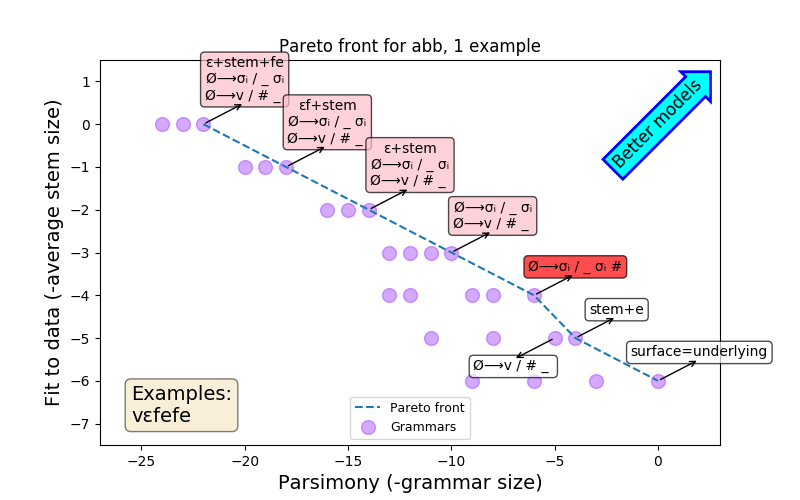
\includegraphics[width = 0.5\textwidth]{abb1.png} 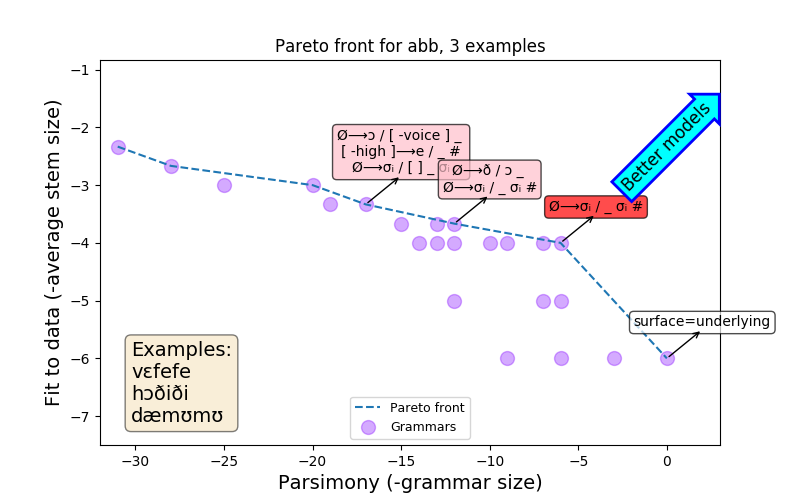
\includegraphics[width = 0.5\textwidth]{abb3.png}
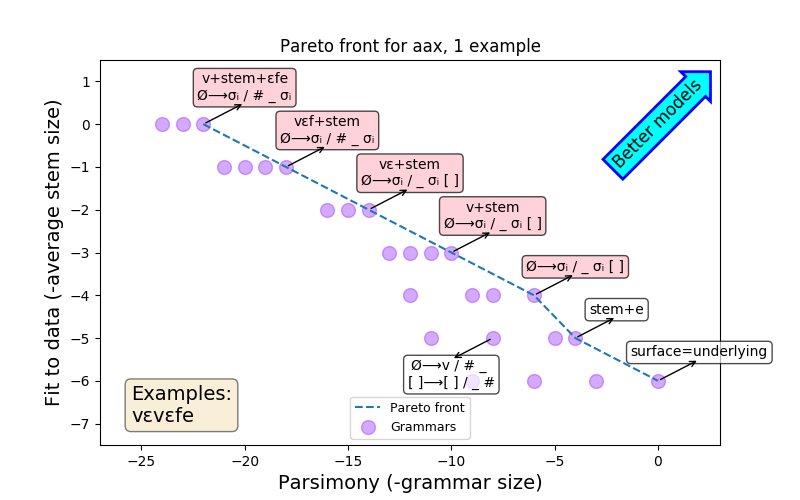
\includegraphics[width = 0.5\textwidth]{aax1.png} 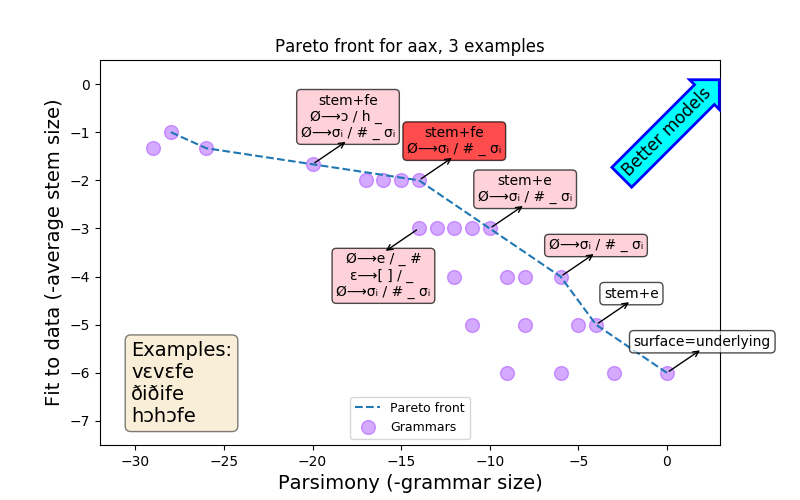
\includegraphics[width = 0.5\textwidth]{aax3.png}
  
  \caption{Pareto fronts for ABB  (Marcus~1999; top two) \& AAX  (Gerken~2006; bottom two) learning problems fo either one example word (left column) or three example words  (right column). {\color{red}Red shade}: ground truth grammar. {\color{red!60}Pink shade}: shares structure with ground truth grammar. White shade: incorrect generalizations. As the number of examples increases, the Pareto fronts develop a sharp kink around the ground truth grammar, which indicates a stronger preference for the correct grammar. With one example the kinks can still exists but are less pronounced.}\label{quadrupleFrontier}
\end{figure}

\subsection{Beyond artificial grammars: Applying BPL to natural language}

A successful model of
artificial grammar learning should also explain at least some aspects of first language acquisition.
As a first step in this direction,
we take the same model that we applied to
these AGL learning problems and use it to solve phonology textbook exercises.
Each of these textbook exercises is an inductive reasoning
problem where the learner must
explain surface pronunciations
in terms of a latent generative model (a program).
Figure~\ref{naturalLanguageExample}
shows our model solving a
representative textbook problem.

\textbf{TIM: Should I talk about UG? We needed it for Tibetan. We probably don't have space.}


\begin{figure}\centering
  \begin{minipage}{7cm}\centering
    \textbf{Textbook Tibetan counting problem:}
    \begin{tabular}{ll}\toprule
Number & Surface form
\\ \midrule
10 & \textipa{d\super Zu}\\
1 & \textipa{d\super Zig}\\
11 & \textipa{d\super Zugd\super Zig}\\
4 & \textipa{Si}\\
%14 & \textipa{d\super ZubSi}\\
40 & \textipa{Sibd\super Zu}\\
9 & \textipa{gu}\\
19 & \textipa{d\super Zurgu}\\
%90 & \textipa{gubd\super Zu}\\
5 & \textipa{Na}\\
%15 & \textipa{d\super ZuNa}\\
%50 & \textipa{Nabd\super Zu}\\
\bottomrule
\end{tabular}
  \end{minipage}%
  \hspace{0.5cm}%
  \begin{minipage}{6cm}\centering
    \textbf{Our model's solution:}
    
    Induced phonological rule: \texttt{C}$\to\varnothing /$\texttt{\#\_C} \\
    \hspace{0.5cm}\emph{(Reduce word initial consonant clusters)}

    Induced underlying representations:
\\\begin{tabular}{ll}\toprule
1 & \textipa{gd\super Zig}\\
4 & \textipa{bSi}\\
5 & \textipa{Na}\\
9 & \textipa{rgu}\\
10 & \textipa{bd\super Zu}
\bottomrule
\end{tabular}    
  \end{minipage}
  \caption{Example textbook phonology exercise (left) and the solution our model discovers for it (right). To solve this problem the model must jointly infer unobserved underlying representations for each of the Tibetan numbers, along with a phonological rule that explains their surface pronunciations. The same code that calculated the Pareto fronts (Figure~\ref{quadrupleFrontier}) produces this analysis of the Tibetan count system.}\label{naturalLanguageExample}
  \end{figure}






%\pagebreak
%% \begin{figure}
%%   \begin{tikzpicture}
%%     %  \draw[help lines] (0,0) grid (10,-10);
%%     \node(UG)[purple,align = center,rotate = 90] at (1,-1) {\textbf{Universal}\\\textbf{Grammar}};
%%     %\draw[ultra thick] (2,0) rectangle (13,-2.3);


%%     \node(sounds) at (7,-0.3) {Phoneme Inventory};
%%     \node(soundExamples)[draw,align = center] at (7,-1.3) {\textipa{@, p, E, 2, k}\\\textipa{a, 3, A, O, d}\\$\cdots$};

%%     \node at (11,-0.3) {Program space};
%%     \node(programSpace)[draw,align = left] at (11,-1.3) {$\mathcal{M}\to \mathcal{A} | $\verb|stem|$|\mathcal{M}+\mathcal{M}$\\$\mathcal{P}\to \mathcal{R}\circ \mathcal{R}\circ \cdots \circ \mathcal{R}$};

%%     \node(featureSpace) at (3.5,-0.3) {Feature space};
%%     \node(featureExamples)[draw,align = center] at (3.5,-1.3) {\verb|voiced|, \verb|vowel|\\\verb|obstruent|, \verb|nasal|\\$\cdots$};

%%     \draw[thick,->] (featureExamples.east) -- (soundExamples.west);
%%     \draw[thick,->] (soundExamples.east) -- (programSpace.west);


%%     \node(universalBox)[purple,draw,ultra thick, fit = (sounds) (featureSpace) (featureExamples) (soundExamples) (programSpace)] {};
%%     \draw(lowerCausalArrow)[thick,->] (featureExamples.south) .. controls (7,-2.5) ..  (programSpace.south);

%%     \node(morphology)[blue,align = above,rotate = 90] at (1,-5) {\textbf{Programs}};
%%     \draw[ultra thick,->] (UG.west) -- (morphology.east);

%%     \node(ABAmorphologyLabel) at (10.5,-3.5) {Pig Latin Morphology};
%%     \node(ABAmorphology) [draw,align = left] at (10.5,-4){ \verb|observation|$\to$\verb|stem|};

%%     \node(ABAphonologyLabel) at (10.5,-5.3) {Pig Latin Phonology};
%%     \node(ABAphonology) [draw,align = left] at (10.5,-6.3) {%
%% $r_1$:      $\varnothing\to$\verb|C|$_i$ $/$ \verb|#C|$_i$\verb| [ ]* _ #|\\%
%%       $r_2$:      $\varnothing\to$ \textipa{e} $/$ \verb| _ #|\\%
%%     $r_3$: \verb|C|$\to\varnothing$ $/$ \verb|# _|};
%%     \node(ABAmorphologyBox)[blue,draw,ultra thick, fit = (ABAmorphologyLabel) (ABAphonology)] {};
    
%%     %  \draw[ultra thick] (2,-3) rectangle (7,-7);

%%     \node(polishMorphologyLabel) at (4.5,-3.5) {Polish Morphology};
%%     \node(polishMorphology) [draw,align = left] at (4.5,-4.3) {\verb|singular|$\to$ \verb|stem|\\\verb|plural|$\to$ \verb|stem|$ + $ /\textipa{i}/};

%%     \node at (4.5,-5.5) {Polish Phonology};
%%     \node(polishPhonology) [draw,align = left] at (4.5,-6.3) {%
%%       $r_1$: \textipa{o}$\to$\textipa{u}$/$\verb|_[-nasal +voice]#|\\%
%%       $r_2$: \verb|[-sonorant]|$\to$\verb|[-voice]|$/$\verb|_#|};
%%     \node(polishMorphologyBox)[blue,draw,ultra thick, fit = (polishMorphologyLabel) (polishPhonology)] {};

%%     \draw[ultra thick,->] (universalBox.south) -- (ABAmorphologyBox.north);
%%     \draw[ultra thick,->] (universalBox.south) -- (polishMorphologyBox.north);
    
%%     \node(lexicon)[magenta,align = center,rotate = 90] at (1,-10) {\textbf{Words}};
%%     \draw[ultra thick,->] (morphology.west)-- (lexicon.east);

%%     \node(p1) [align = left] at (9.5,-8) {\verb|LATIN:| \textipa{l\ae tIn}};
%%     \node(p2) [draw,align = left] at (9.5,-9.5) {\textipa{l\ae tIn}\nextForm{r_1}\\\textipa{l\ae tInl}\nextForm{r_2}\\\textipa{l\ae tInle}\nextForm{r_3}\\\textipa{\ae tInle}}; %\\\textipa{l\ae tInle}}};
%%     \draw [thick,->] (p1.south) -- (p2.north);
    
%%     \node(w1) [align = left] at (12,-8) {\verb|ASK:| \textipa{\ae sk}};
%%     \node(w2) [draw,align = left] at (12,-9.5) {\textipa{\ae sk}\nextForm{r_1}\\\textipa{\ae sk}\nextForm{r_2}\\\textipa{\ae ske}\nextForm{r_3}\\\textipa{\ae ske}};
%%     \draw [thick,->] (w1.south) -- (w2.north);
    
%%     \node[magenta,draw,align= left](ABAvocabulary) at (10.5,-11.5){\textipa{\ae tInle}, \textipa{\ae ske}, $\cdots$ };
%%     \draw [thick,->] (p2.south) -- (ABAvocabulary.north);
%%     \draw [thick,->] (w2.south) -- (ABAvocabulary.north);
%%     \node(ABAlexiconBox)[draw,ultra thick, fit = (p1) (w1) (ABAvocabulary)] {};
%%     \draw [ultra thick,->] (ABAmorphologyBox.south) -- (ABAlexiconBox.north);  

%%     \node(crib) at (4.5,-8) {\verb|horn:| \textipa{rog}};
%%     \node(Cingular)[draw,align = left] at (3.5,-9.5) {\verb|singular:|\\ \textipa{rog}\nextForm{r_1}\\\textipa{rug}\nextForm{r_2}\\\textipa{ruk}};
%%     \node(plural)[draw,align = left] at (5.5,-9.5) {\verb|plural:|\\ \textipa{rogi}\nextForm{r_1}\\\textipa{rogi}\nextForm{r_2}\\\textipa{rogi}};
%%     \draw [thick,->] (crib.south) -- (Cingular.north);
%%     \draw [thick,->] (crib.south) -- (plural.north);

%%     \node[magenta,draw,align = left] (polishObservation) at (4.5,-11.5) {\verb|horn, singular:| \textipa{\v{z}wop}\\\verb|horn, plural:| \textipa{\v{z}wubi}};
%%     \draw [thick,->] (Cingular.south) -- (polishObservation.north);
%%     \draw [thick,->] (plural.south) -- (polishObservation.north);

%%     \node(polishLexicon)[draw,ultra thick, fit = (crib) (Cingular) (plural) (polishObservation)] {};
%%     \draw [ultra thick,->] (polishMorphologyBox.south) -- (polishLexicon.north);
    
%%   \end{tikzpicture}
%% \end{figure}


%\bibliographystyle{named}
\bibliographystyle{unsrt} \bibliography{main}

\pagebreak
\section{Appendix}



\begin{table*}[h]
\centering
\begin{tabular*}{\textwidth}{ll}
\toprule
Grammar rule  & English description \\\midrule
$\mathcal{P}\to \mathcal{R}\circ \mathcal{R}\circ \cdots \circ \mathcal{R}$&Phonology $\mathcal{P}$ is a sequence of compositions of rewrites $\mathcal{R}$\\
$\mathcal{R}\to \mathcal{F}\longrightarrow \mathcal{C} / \mathcal{T}\_\mathcal{T}$& Rewrite focus $\mathcal{F}$ to structural change $\mathcal{C}$ between triggers $\mathcal{T}$\\
$\mathcal{T}\to \# \mathcal{T}' | \mathcal{T}'$ & Triggers optionally match end of string\\
$\mathcal{T}'\to \epsilon | \mathcal{X} \mathcal{T}' | \mathcal{X}^* \mathcal{T}'$ & Triggers are sequences of matrices $\mathcal{X}$ possibly with Kleene star\\
$\mathcal{X}\to a|t|s|\cdots$&Matrices can be constant phonemes\\
$\mathcal{X}\to [\pm \mathcal{G} \; \pm \mathcal{G} \; \cdots \; \pm \mathcal{G}]$& Matrices check features $\mathcal{G}$\\
$\mathcal{X}\to \sigma$&Matrices can be whole syllables\\
$\mathcal{G}\to \text{voice}|\text{nasal}|\cdots$&Standard phonological features\\
$\mathcal{F}\to \mathcal{X}$&Focus can be a feature matrix\\
$\mathcal{F}\to \varnothing$&Focus can be empty (insertion rule)\\
$\mathcal{F}\to\mathbb{Z}$&Focus can be one of the triggers (copies it)\\
$\mathcal{C}\to\mathcal{X}$&Structural change can be a feature matrix\\
$\mathcal{C}\to\varnothing$&Deletion rule\\
\bottomrule
\end{tabular*}
\caption{Grammar over phonologies. The non-terminal $\mathcal{P}$ is the start symbol for the grammar.}
\label{phonologyGrammar}
\end{table*}

\begin{table*}[h]
\centering
\begin{tabular*}{\textwidth}{ll}
\toprule
Grammar rule  & English description \\\midrule
$\mathcal{W}\to (\mathcal{M}) \mathcal{M} (\mathcal{M})$&Morphology builds words $\mathcal{W}$ by concatenating morphemes $\mathcal{M}$. Prefix/Suffix optional (in parentheses)\\
$\mathcal{M}\to$ sequence of phonemes\bottomrule
\end{tabular*}
\caption{Grammar over morphologies. The non-terminal $\mathcal{W}$ is the start symbol for the grammar.}
\label{morphologyGrammar}
\end{table*}

\pagebreak
\subsection{Inference}

The solver takes as input:
\begin{itemize}
\item A set of inflected surface forms, $\{x_n\}$. Here the variable $x_n$ refers to all of the inflections of a word. So an example set of 3 inflected surface forms might be $\{(\text{fish},\text{fished}), (\text{walk},\text{walked}), (\text{eat},\text{ate})\}$.
\item A bound on the number of rules to consider synthesizing, $B_R$.
\end{itemize}
It produces as output:
\begin{itemize}
\item A set of underlying forms, $\{u_n\}$.
\item A morphology consisting of a prefix ($\{p_i\}$) and a suffix ($\{s_i\}$)  for each inflection
\item  A sequence of rules, $\{r_j\}_{j = 1}^{B_R}$
\end{itemize}
It is \emph{guaranteed} to discover the rules, morphology, and underlying forms minimizing:
\begin{equation}
  \text{solver}(\{x_n\},B_R) = \argmin_{\{r_j\}_{j = 1}^{B_R}, \{u_n\}, \{p_i\}, \{s_i\}} \sum_j \text{cost}(r_j) + \sum_i (\text{cost}(p_i) + \text{cost}(s_i) ) + \sum_n \text{cost}(u_n)
\end{equation}
In exchange for this strong guarantee, however, it has only a very
weak guarantee on the amount of time it will take to discover the
solution: in the worst case, it will take time exponential size of the
problem. In practice it takes close to a day for it to do exact search over 3 rules.
For easy problems, like the AGL experiments, I can get away with 4 rules if I wait for a few hours.

One can also ask the solver for the top $K$ solutions minimizing the cost function, which I will write:
\begin{equation}
  \text{solver}_K(\{x_n\},B_R) = \text{the }K\text{ minimum cost solutions.}
\end{equation}
One can also provide additional constraints to the solver, for example telling it what the underlying forms are,
or telling it what some of the rules are. I will write these constraints by adding an extra argument to the solver
that looks like conditioning in Bayesian inference. For example,
\begin{equation}
  \text{solver}_K(\{x_n\},B_R|u_1 = \text{fish}) = \text{the }K\text{ minimum cost solutions where }u_1\text{ has to be fish.}
  \end{equation}

So now the game is to leverage this solver as a ``black box'' inside of an incomplete search algorithm.
A key subroutine in my attempts at building such a search algorithm is
\texttt{solveIncrementalChange}, which takes as input an existing set of rules ($\{r_j^e\}_{j = 1}^{B_R}$)
along with a \textbf{search radius} ($R$),
and solves for a solution that changes at most \textbf{search radius} rules.
\begin{equation}
  \text{solveIncrementalChange}_K (\{x_n\}, \{r_j^e\}_{j = 1}^{B_R}, R)
   = \text{solver}_K (\{x_n\}, B_R+1 | r_j\not= r_j^e \text{ at most }R\text{ times})
\end{equation}
So \texttt{solveIncrementalChange} can add a rule (see $B_R+1$). I didn't build in any explicit mechanism for reordering rules -- if you set the search radius $R$ to 2, then it could effectively swap 2 rules.

In addition to synthesizing large programs, we also have to deal with
large data sets. Armando already came up with a nice trick for this called CEGIS\footnote{counterexample
  guided inductive synthesis}.
The idea behind CEGIS is that you synthesize a program from one example,
and then you check to see if that program is inconsistent with any other examples.
If not then you are done.
Otherwise, you have found a \textbf{counterexample}. You add the counterexample to your
training data set and repeat.

Combining \texttt{solveIncrementalChange} with CEGIS gives the
skeleton of the inference algorithm that I have been experimenting
with, called \texttt{incrementalCEGIS}. See the pseudocode at the top of the next page:
\pagebreak
\begin{algorithmic}
  \STATE \textbf{\texttt{incrementalCEGIS}}:
  \STATE {\bfseries Input:} Matrix of inflected forms for $N$ lexemes, $X$
  \STATE {\bfseries Hyperparameter:} Batch size $B$
  \STATE {\bfseries Output:} underlying forms, $\{u_n\}$; prefixes $\{p_i\}$; suffixes $\{s_i\}$; rules $\{r_j\}$
  \STATE // Initialize training set $T$ with $B$ examples
  \STATE Set $T = $ inflections for $B$ lexemes in $X$
  \STATE // Find a solution for examples, using as many rules as you need ($\infty$)
  \STATE Set $\{r_j\}_{j = 1}^{B_R}, \{p_i\}, \{s_i\} = \text{solver}(T,\infty)$
  \REPEAT
  \STATE // Find the set of counterexamples $C$ inconsistent with our current guess as to what the solution is
  \STATE Set $C = \{x | x\in X \text{ and } x \text{ inconsistent with } \{r_j\}_{j = 1}^{B_R},\{p_i\}, \{s_i\}\}$
  \STATE // If there are no counterexamples as we are done
  \STATE \textbf{if} $C = \varnothing$ \textbf{ then return }$\{r_j\}_{j = 1}^{B_R},\{p_i\}, \{s_i\}$
  \STATE // Add a batch of counterexamples to the training set
  \STATE $T\gets T\cup \{C_j\}_{j = 1}^B$
  \STATE // Start out with a search radius of $1$ and increase it until we find a way of accommodating another example
  \FOR{$R = 1,2,3,4,...$}
%  \FOR {$c\in C$}
  \STATE Set synthesisResult$ = \text{solveIncrementalChange}(T,\{r_j\},R)$
  \IF{synthesisResult$\not= \bot$}
  \STATE Set $\{r_j\}_{j = 1}^{B_R}, \{p_i\}, \{s_i\} = $synthesisResult
  \STATE \textbf{break out of loop over }$R$ // Successfully updated both our solution and the training set
\end{algorithmic}
\vspace{1cm} 

One important feature of this approach is that it does not reuse
previous inferences about the morphology or the underlying forms.
I think we want to add this.
For example, we might allow it to change up to $R$ underlying forms,
or disallow changes in the morphology once the training set is big enough.

Variations of \textbf{incrementalCEGIS} that I have tried:
\begin{itemize}
\item[] Maintaining a population of solutions. Instead of taking the top 1 solution every time you synthesize, try taking the top $K$. There is some trade-off here between the cost of solving for more solutions and
  the benefit of not needing as many counterexamples. I have not done any systematic experiments,
  but my general sense is that this trade-off favored $K = 1$ in practice (so not maintaining a population of solutions).
\item[] Letting the solver insert the new rule anywhere vs constraining it to either append or prepended the new rule. Sketch uses up a lot of memory whenever I let it insert the rule anywhere -- not sure why this is.
\item[] Giving sketch more problems to solve but making each problem smaller. Here what I do is have an outer loop that iterates over all of the different ways you could edit an existing set of rules, and then invoke the solver for each of these. So for example I invoke the solver telling it to change only the first rule,
  then I invoke it telling it to change only the second rule, etc, finally telling it to keep all the rules the same but add a new rule.
\end{itemize}

\subsection{Search heuristics}

\subsubsection{Guessing underlying forms}

\textbf{incrementalCEGIS} is a generic way of learning large programs that explain large data sets,
and does not encode any domain specific knowledge about phonology.
Empirically, the search problem is \emph{much} easier if you
either know what the underlying forms are or have some constraints on what the underlying forms are.
If I introspect on my own reasoning process while solving these problems,
I usually guess at most a few plausible underlying forms for each lexeme.
I encoded a simple heuristic for guessing parts of underlying representations:
given prefixes/suffixes $\left\{p_i \right\}$ \& $\left\{s_i \right\}$
and observed inflections for a single lexeme $\left\{x_i \right\}$,
this heuristic guesses that the underlying form begins with the longest shared prefix
of the surface forms with the prefixes chopped off,
and that it ends with the longest shared suffix of the surface forms with the suffixes chopped off.
For example, if we have surface forms $(\text{test},\text{testing},\text{tests})$,
and have prefixes $(\text{t},\text{t},\text{t})$ and suffixes $(\text{t},\text{ting},\text{ts})$,
this heuristic constrains the underlying form to start with $\text{es}$ and end with $\text{es}$.



\section{Related work}

Minimum generalization learner: \cite{Albright03rulesvs}. The interesting similarity here is that we both learned the structure of the rules. But it's restriction to the supervised case hampers its ability to really capture what a grammar is about (a generative model learned without supervision) and it misses out on lots of cool phenomena.

Maximum entropy learner:~\cite{goldwater2003learning}. Whether you take an OT perspective or a generative perspective, the structure of the rules (or constraints) has to come from somewhere. How do you learn that structure? This is a program induction problem.

Unsupervised phonological rule learners:
~\cite{cotterell-peng-eisner-2015} learns weighted fst's while
\cite{rulebased} learns context-sensitive rewrites. Here we show that
these results and more can be reformulated as a program induction
problem, and that doing so buys you (1) connections to probabilistic
programming and Bayesian program learning; (2) theoretical guarantees;
(3) a bunch more phenomena modeled, like supervised cases (pig latin),
UG, and infant studies.

References from a discussion with Adam Albright:

LISA (an acronym standing for something) babbling

Alex Cristia: Can infants learn phonology in the lab?

David Stampe: Spontaneous Devoicing. Evidence of UG

Chapter 8 of SPE~\cite{chomsky1968sound}: What is the right evaluation metric for rules?

Collin Wilson: paletization generalizations as more evidence of UG in phonology

Degree of articulatory effort as an inductive bias

Rules shouldn't be too disruptive of the underlying form. Should also minimize confuseability. Final devoicing is a good example of this. PMAP. ``weak contrast''


\section{Experiments}

\subsection{Phonological Rule Induction}

Several metrics of success here: (1) how well does it compress the
data? (2) how well does it predict held out forms? (3) how natural or
interpretable are the resulting solutions?

Here are cases where I think it learns something cool:

\noindent\begin{tabular*}{\textwidth}{lclll}
  \toprule
  Language&Example data&Underlying forms&Phonology&Phenomena\\\midrule
Gen&
\begin{tabular}{l}
\textipa{sra}\\
\textipa{agble}\\
\textipa{drE}\\
\textipa{hlE}
\end{tabular}
&\textipa{l} underlying
  & \textipa{l}$\to$\textipa{r}$/$\verb|[+coronal] _|
  &
\textipa{l}$\sim$\textipa{r} alternation
  \\
  \bottomrule  \end{tabular*}

\noindent\begin{tabular*}{\textwidth}{lclll}
  \toprule
  Language&Example data&Phonology&Morphology&Phenomena\\\midrule
  Tibetan&
\begin{tabular}{ll}
1&\textipa{\|x{j}ig}\\
4&\textipa{\|x{s}i}\\
5&\textipa{Na}\\
9&\textipa{gu}\\
10&\textipa{\|x{j}u}\\
11 ($= 10 + 1$) & \textipa{\|x{j}ug\|x{j}ig}\\
14 ($= 10 + 4$) & \textipa{\|x{j}ub\|x{s}i}\\
15 ($= 10 + 5$) & \textipa{\|x{j}uNa}\\
19 ($= 10 + 9$) & \textipa{\|x{j}urgu}\\
40 ($= 4 + 10$) & \textipa{\|x{s}ib\|x{j}u}\\
50 ($= 5 + 10$) & \textipa{Nab\|x{j}u}\\
90 ($= 9 + 10$) & \textipa{gub\|x{j}u}
\end{tabular}
&
\begin{tabular}{l}
  \verb|[-nasal]|$\to\varnothing $ $/$ \verb|# _|\\
  \emph{or,}\\
  \verb|C|$\to\varnothing $ $/$ \verb|# _ C|\\
  \end{tabular}
  &
\emph{given in problem}
  &
Consonant cluster reduction
  \\
  \bottomrule  \end{tabular*}

\begin{tabular*}{\textwidth}{lclll}
  \toprule
  Language&Example data&Phonology&Morphology&Phenomena\\\midrule
  Kerewe&
\begin{tabular}{llll}
\textipa{kubala} & \textipa{kubalana} & \textipa{kubalila} & \textipa{kubalilana}\\
\textipa{kugaya} & \textipa{kugayana} & \textipa{kugayila} & \textipa{kugayilana}\\
\textipa{kub\'ala} & \textipa{kub\'al\'ana} & \textipa{kub\'al\'ila} & \textipa{kub\'al\'ilana}\\\hline
\textipa{kut\'ub\'ala} & \textipa{kuk\'ib\'ala} & \textipa{kut\'ub\'alila} & \textipa{kuk\'it\'ubalila}\\
\textipa{kut\'ug\'aya} & \textipa{kuk\'ig\'aya} & \textipa{kut\'ug\'ayila} & \textipa{kuk\'it\'ugayila}\\
\textipa{kut\'ub\'ala} & \textipa{kuk\'ib\'ala} & \textipa{kut\'ub\'alila} & \textipa{kuk\'it\'ubalila}
\end{tabular}
&
\begin{tabular}{l}
  \verb|[]|$\to$\verb|[-H]|$/$\verb|[+H] [] _| \\
  \verb|[]|$\to$\verb|[+H]|$/$\verb|[+H] [] _ []|
  \end{tabular}
  &
\begin{tabular}{ll}
\textipa{ku}$+$stem$+$\textipa{a}\\
\textipa{ku}$+$stem$+$\textipa{ana}\\
\textipa{ku}$+$stem$+$\textipa{ila}\\
\textipa{ku}$+$stem$+$\textipa{ilana}\\
\textipa{kut\'u}$+$stem$+$\textipa{a}\\
\textipa{kuk\'i}$+$stem$+$\textipa{a}\\
\textipa{kut\'u}$+$stem$+$\textipa{ila}\\
\textipa{kuk\'it\'u}$+$stem$+$\textipa{ila}
  \end{tabular}
  &
\begin{tabular}{ll}
  Tone spreading\\
  Rule ordering
  \end{tabular}
  \\
  \bottomrule  \end{tabular*}

\noindent\begin{tabular*}{\textwidth}{lclll}
  \toprule
  Language&Example data&Phonology&Morphology&Phenomena\\\midrule
  Polish&
\begin{tabular}{ll}
\textipa{dom} & \textipa{domi}\\
\textipa{kot} & \textipa{koti}\\
\textipa{lut} & \textipa{lodi}\\
\textipa{vus} & \textipa{vozi}\\
\textipa{wuk} & \textipa{wugi}\\
\textipa{ruk} & \textipa{rogi}\\
\textipa{bur} & \textipa{bori}\\
\textipa{\|x{s}um} & \textipa{\|x{s}umi}
\end{tabular}
&\begin{tabular}{l}
   \textipa{o}$\to$\textipa{u}$/$\verb|_[-nasal +voice]#|\\%
\verb|[-sonorant]|$\to$\verb|[-voice]|$/$\verb|_#|
   \end{tabular}
  &
\begin{tabular}{ll}
  stem\\
  stem$ + $\textipa{i}
  \end{tabular}
  &
\begin{tabular}{ll}
  Final devoicing\\
  Rule ordering
  \end{tabular}
  \\
  \bottomrule  \end{tabular*}

\noindent\begin{tabular*}{\textwidth}{lclll}
  \toprule
  Language&Example data&Phonology&Morphology&Phenomena\\\midrule
Makonde  &
\begin{tabular}{lll}
\textipa{am\'aNga} & \textipa{am\'ile} & \textipa{\'ama}\\
\textipa{ak\'aNga} & \textipa{ak\'ile} & \textipa{\'aka}\\
\textipa{av\'aNga} & \textipa{av\'ile} & \textipa{\'ova}\\
\textipa{am\'aNga} & \textipa{am\'ile} & \textipa{\'oma}\\
\textipa{ut\'aNga} & \textipa{ut\'ile} & \textipa{\'uta}\\
\textipa{av\'aNga} & \textipa{av\'ile} & \textipa{\'eva}\\
\textipa{tav\'aNga} & \textipa{tav\'ile} & \textipa{t\'ava}\\
\textipa{uNg\'aNga} & \textipa{uNg\'ile} & \textipa{\'uNga}\\
\textipa{pat\'aNga} & \textipa{pat\'ile} & \textipa{p\'ota}
\end{tabular}
&
\begin{tabular}{l}
\verb|[]|$\to$\verb|[-stress]| $/$ \verb| _ [ ]* [ +stress]|\\
\verb|[+middle -stress]|$\to$\textipa{a}$/$\verb| _ [ ]|
  \end{tabular}
  &
\begin{tabular}{ll}
  stem$ + $\textipa{\'aNga}\\
  stem$ + $\textipa{\'ile}\\
  stem$ + $\textipa{a}
  \end{tabular}
  &
\begin{tabular}{ll}
Stress patterns\\
Neutralizing rule
  \end{tabular}
  \\
  \bottomrule  \end{tabular*}

\noindent\begin{tabular*}{\textwidth}{lclll}
  \toprule
  Language&Example data&Phonology&Morphology&Phenomena\\\midrule
  Kikuria&
\begin{tabular}{ll}
\textipa{rema} & \textipa{remera}\\
\textipa{roma} & \textipa{romera}\\
\textipa{tiga} & \textipa{tegera}\\
\textipa{ruga} & \textipa{rogera}\\
\textipa{hoora} & \textipa{hoorera}\\
\textipa{siika} & \textipa{seekera}\\
\textipa{huuta} & \textipa{hootera}\\
\textipa{suraaNga} & \textipa{suraaNgera}
\end{tabular}
&
\verb|[+high]|$\to$\verb|[+middle]|$ /$\verb| _ [-low]* [+middle]|
  &
\begin{tabular}{ll}
  stem$ + $\textipa{a}\\
  stem$ + $\textipa{era}
  \end{tabular}
  &
Vowel harmony
  \\
  \bottomrule  \end{tabular*}

\noindent\begin{tabular*}{\textwidth}{lclll}
  \toprule
  Language&Example data&Phonology&Morphology&Phenomena\\\midrule
  Hungarian&
  \begin{tabular}{llll}
\textipa{a:g\super y} & \textipa{a:g\super yban} & \textipa{a:k\super yto:l} & \textipa{a:g\super ynak}\\
\textipa{\"o:r} & \textipa{\"o:rben} & \textipa{\"o:rt\"o:l} & \textipa{\"o:rnek}\\
\textipa{ku:t} & \textipa{ku:dban} & \textipa{ku:tto:l} & \textipa{ku:tnak}\\
\textipa{re:s} & \textipa{re:zben} & \textipa{re:st\"o:l} & \textipa{re:snek}\\
\textipa{rab} & \textipa{rabban} & \textipa{rapto:l} & \textipa{rabnak}\\
\textipa{vi:z} & \textipa{vi:zben} & \textipa{vi:st\"o:l} & \textipa{vi:znek}\\
\textipa{fal} & \textipa{falban} & \textipa{falto:l} & \textipa{falnak}\\
\textipa{test} & \textipa{tezdben} & \textipa{testt\"o:l} & \textipa{testnek}
  \end{tabular}&
  \begin{tabular}{l}
    \verb|V|$\to$\verb|[+mid +tense +front]|$ /$\\\verb|  [ +front ] [ ]* _ |\\
         \verb|[ ]|$\to$\verb|[+voice]|$ / $\\\verb| _ [+bilabial]|\\
         \verb|[-sonorant]|$\to$\verb|[-voice]|$ / $\\\verb| _ [-voice]|
    \end{tabular}
  &
  \begin{tabular}{l}
    stem\\
    stem$ + $\textipa{ban}\\
    stem$ + $\textipa{to:l}\\
    stem$ + $\textipa{nak}
  \end{tabular}
  &
  \begin{tabular}{l}
    Vowel harmony\\
    Voicing assimilation\\
    Rule ordering
    \end{tabular}
  \\
\bottomrule  \end{tabular*}

\pagebreak
These problems are solved:
\begin{itemize}
\item Kikurai: fricatives alternate with stops after nasals
\item Greek: Velar stops alternate with palletized versions before front vowels
\item Farsi: Trills alternate with flaps
\item Osage: coronal stops become dentals before central vowels
\item Amharic: alternation between \textipa{@} \& \textipa{E}
\item Gen: l/r alternation
\item Kishambaa: voiced/unvoiced nasals alternate
\item  Thai: stops are unreleased word finally
\item Palauan: a word initial neutralizing rule
\item Quechua: Velar becomes uvular when followed by uvular (spreading)
\item Lhasa Tibetan: no contrast between velar/uvular, or voiced/voiceless stops or fricatives
\item Axininca Campa: stops become glides
\item Kikuyu: infinitive prefix can surface as either k or \textipa{G}
\item Korean: vowel harmony, aspiration only surfaces in certain contexts
\item Hungarian: vowel harmony and voicing assimilation
\item Kikuria: vowel harmony
\item Farsi: a deletion rule explains singular/plural
\item Tibetan: initial consonant cluster reduction explains counting system
\item Makonde: stress patterns; unstressed vowels are neutralized
\item North Saami: 3 neutralization rules explain nominative sg essive
\item Samoan: 2 deletion rules that explain words that sound the same in one inflection being different in another
\item     Russian: devoicing of word final obstruent
\item English: verbal inflections (voicing assimilation, epenthesis)
\item Finnish: nominative/partive explained by vowel raising and vowel harmony
\item Kerewe: Interacting tone rules
\item Polish: vowel alternations interacting with devoicing of word final obstruent in singular/plural
\item Ancient Greek: voicing assimilation, deaspiration, deletion rule. Order matters.
\item Serbo-Croatian: predictable stress, devoicing, neutralizing, epenthesis
\end{itemize}
17 textbook problems are not solved. 2 of these need a tier-based representation. A couple more of these are due to limitations in the program learner's representation of rules. The rest are because they involve scaling to more than 3 rules, which is about the practical limit for exact search with these methods.
\pagebreak


\subsubsection{An approximation to UG: Program fragments}

Within-rule reuse of structure:
\begin{tabular}{ll}
  Tibetan: & {\color{red}\texttt{C}}$\to\varnothing /$\verb|#_|{\color{red}\texttt{C}} \\
  English: &          \verb|[-sonorant]|$\to${\color{red}\texttt{[-voice]}}$ / ${\color{red}\texttt{[-voice]}}\verb| _ |\\
Kikuria: &\verb|[ +high ]|$\to$ {\color{red}\texttt{[ +middle ]}} $/$ \verb| _ [ -low ]*| {\color{red}\texttt{[ +middle ]}}
\end{tabular}

\vspace{0.5cm}\noindent Within-language reuse of structure:
\begin{tabular}{ll}
  Axininca Campa: &
  \begin{tabular}{l}
    \textipa{p}{\color{red}$\to$}\textipa{w} {\color{red}$/$ \texttt{[ ] \_}}\\
    \textipa{k}{\color{red}$\to$}\textipa{y}\, {\color{red}$/$ \texttt{[ ] \_}}
  \end{tabular}\\
  English:&
  \begin{tabular}{l}
    {\color{red}$\varnothing\to$\textipa{@} $/$} \verb|[+sib] _ [+sib]|\\
    {\color{red}$\varnothing\to$\textipa{@} $/$} \verb|[+cor +stop] _ [+cor +stop]|
  \end{tabular}
\end{tabular}


\vspace{0.5cm}\noindent Cross-language reuse of structure:
\begin{tabular}{ll}
  Russian/Polish:& \verb|[-sonorant]|$\to$\verb|[-voice]|$/$\verb|_#|\\
  Samoan/Tibetan:&
  \begin{tabular}{l}
    {\color{red}\texttt{C}$\to\varnothing /$}\verb|_#|\\
    {\color{red}\texttt{C}$\to\varnothing /$}\verb|#_C|
  \end{tabular}\\
  Ancient Greek/Hungarian:&
  \begin{tabular}{l}
    {\color{red}\texttt{[-sonorant]}$\to$\texttt{[-voice}} \texttt{-aspirated]} {\color{red} $/$ \texttt{ \_ [-voice]}}\\
    {\color{red}\texttt{[-sonorant]}$\to$\texttt{[-voice}} \texttt{]} {\color{red} $/$ \texttt{ \_ [-voice]}}
    \end{tabular}
  \end{tabular}

\begin{figure}[h]
  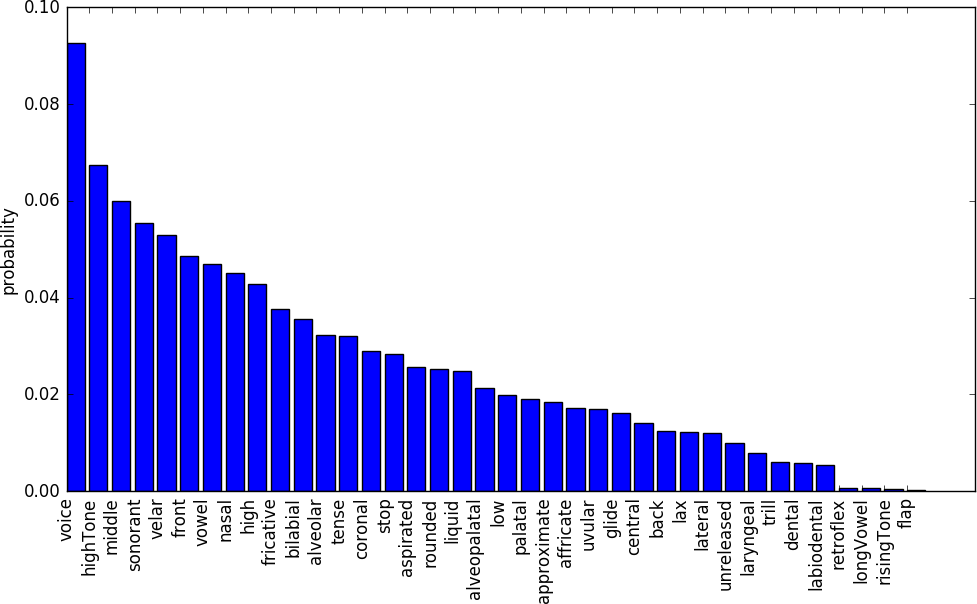
\includegraphics[width = \textwidth]{featureFrequencies.png}
  \caption{Which features are frequently used in correct rules? Voicing, sonorant, nasality are very frequent, and are also near the top of the feature geometry hierarchy. Feature geometry was not given to the system, but you can see at least this coarse level of structure emerge from the data. Vowel features also frequent due to vowel harmony occurring in lots of languages.}
\end{figure}

\begin{figure}[h]
  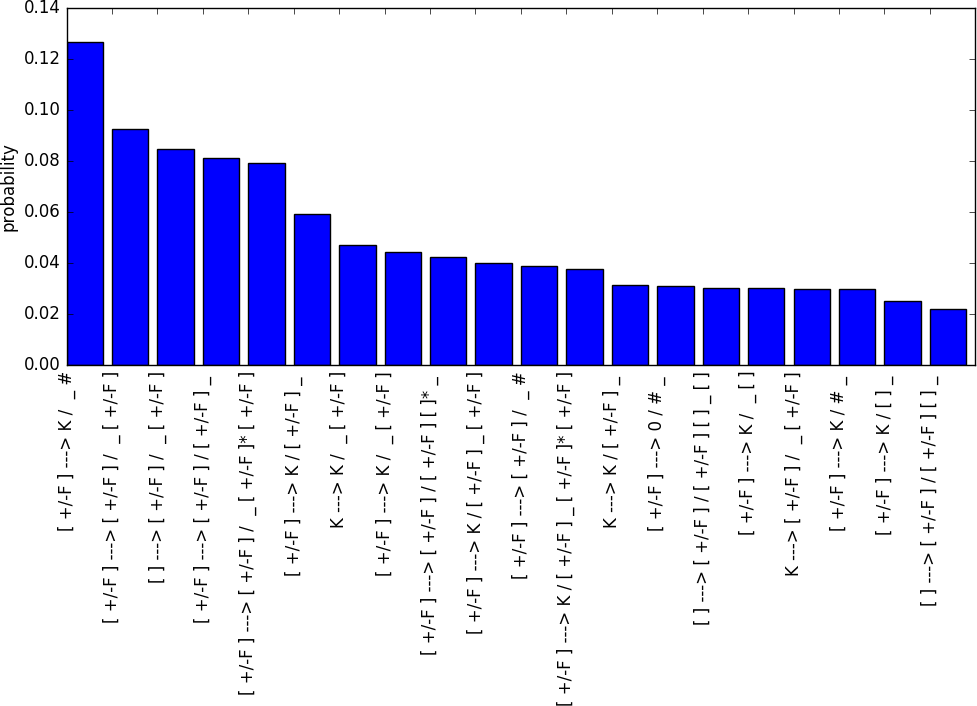
\includegraphics[width = \textwidth]{skeletonFrequencies.png}
  \caption{What is the general structure of rules that occur in phonology, ignoring the particular constants that occur in the rule? Here $K$ stands in for an arbitrary phoneme; $\pm$features stands in for an arbitrary feature matrix. From this plot you can glean that (1) neutralizing rules are very common (top two most frequent rules); (2) harmony/assimilation rules are also frequent; (4) deletion rules tend to occur at word boundaries. There are about $5\times 10^4$ possible syntactic structures for rules, but only 15 are actually attested (relative frequency$ > 1$). Here I think that the sparsity of the problem sets is hurting us: these results come from 26 problems, so the fact that you see only 15 general schemas isn't too crazy if you don't believe in strong innate constraints on the structure of rules. But looking at this data you also see a generalization that holds across all of the rules learned: the structures tend to be pretty small, so you never see a rule that checks feature values of more than two adjacent segments.}
\end{figure}



%% \subsection{Historical productivity}

%% There is an interesting tension between discovering regularities
%% that are psychologically real (like things that are used productively)
%% and discovering regularities that are in the data but only due to
%% historical accidents. Our system cannot distinguish them.

%% Are these deep analyses real? We don't answer this question, but we do
%% raise it. We are agnostic. These are the kinds of regularities that a
%% good linguist would notice, and our system notices them too.

\subsection{Artificial Phonologies}

It would be cool to model all of the grammars in~\cite{frank2011three}. Right now we can model AAB/ABA patterns like in Gary Marcus's famous infant experiments. Other infant studies with artificial grammars:~\cite{gerken2006decisions}. MNPQ problem:~\cite{smith1966grammatical}.

Analogs in real languages: agreement morphology (eg gender in Spanish
- there is a constraint that two things have to be the same);
reduplication (this could literally be modeled using the same ABA
system); obligatory contour principle (opposite of harmony - two
things have to be different, just like the ssd/sds distinction).

For any of these problems, there is a trade-off between how
complicated of a program you are willing to use and how badly you want
to compress the data. Here, compressing the data means representing
the surface forms with short underlying representations. This
trade-off is of course present in the phonology problem sets as well.
But the problem sets are complicated and have lots of data, precluding
any in-depth analysis of the trade-off except quantitatively. For
these synthetic grammar learning problems, we can dig in and see
exactly what the trade-off looks like for different amounts of data.
See figure~\ref{fronts} for an analysis of this trade-off along with
examples of what the programs look like.



\section{Applications}
The point of this is to motivate why you would want to solve exactly
this problem even though it doesn't do anything more immediately
useful than solve your phonology homework. Practical applications that could come from this line of work:

\begin{itemize}
\item Low-resource language acquisition: \url{http://sapience.dec.ens.fr/bootphon/} for some languages there is very little data and very few speakers
\item Mathematica for Phonology: a lot of the time physicists don't do
  integrals; they just punch them into Mathematica. This is a tool
  that provably finds the ``best'' grammar for some data, sort of like
  how Mathematica finds the correct integral of some expression. And
  just like some integrals are beyond the reach of computer algebra
  systems, some data sets might be beyond the reach of this
  hypothetical tool. Analogy to the work
  in~\cite{schmidt2009distilling}. According to Tim it would be more
  practical for the field for knowledge is to have a system that can
  work out the consequences of a given rule set, maybe pointing out
  places where it's inconsistent with the data or suggesting
  underlying forms. These alternative uses could also be accommodated.
\item A probe for UG: the prior over phonology is a parameter of the
  algorithm which you could in principle estimate from the data or
  compare different settings of the prior to see how well they
  compress the data. Or, come up with the right constraints so that
  the system doesn't generalize in the same places where humans don't
  generalize (surfeit of the stimulus:~\cite{becker2011surfeit}). You
  can approach universal grammar from two directions: what do I need
  to build then so that it will learn the same things that humans
  learn? And what do I need to take out in order to stop it from
  learning things that humans never learn? 
\end{itemize}

\section{Discussion}

Deep learnability issue: what is the actual computational complexity
of learning these grammars? The actual hardness is an empirical
question which you can upper bound by coming up with better heuristics
for inducing grammars. Attempts at \emph{lower bounding} the
complexity of learning has generally been way too conservative. We
want to know the actual hardness of the learning problem, and
constructing a practical program learner shows that it might not be
too hard with the right UG.

We must emphasize that there is \textbf{no general-purpose
  learner}. So we need UG. This tool lets us dig in and study it.
There's always going to be a trade-off between how much you build in and how much data/computation is needed to recover the correct generalizations. Our compromise in the space of this trade-off is to:
\begin{itemize}
\item  Not play in the space of arbitrary turing machines but instead search through a finite program space (bounded program size runtime and memory consumption; program structure given by a grammar)
  \item Make contentfull proposals about what the structure of
    universal grammar might be, and test them empirically on many
    languages
\end{itemize}

\textbf{Comparison with deep learning:} In a sense this project is like
the opposite of deep learning. It's about the kind of learning that
yields explanations of the causal processes behind data sets; where
the learner comes equipped with explicit background knowledge (UG)
that we can tweak finely and systematically.

One similarity though is that some of the phenomena we model, like
infant learning of synthetic grammars, are the sort of things that
humans pick up unconsciously. A lot of deep learning might be
analogous to humans rote learning some motor or perceptual task.


\end{document}
